%%%%%%%%%%%%%%%%%%%%%%%%%%%%%%%%%%%%%%%%%
% Szablon pracy dyplomowej
% Wydział Informatyki 
% Zachodniopomorski Uniwersytet Technologiczny w Szczecinie
% autor Joanna Kołodziejczyk (jkolodziejczyk@zut.edu.pl)
% Bardzo wczesnym pierwowzorem szablonu był
% The Legrand Orange Book
% Version 5.0 (29/05/2025)
%
% Modifications to LOB assigned by %JK
%%%%%%%%%%%%%%%%%%%%%%%%%%%%%%%%%%%%%%%%%


%----------------------------------------------------------------------------------------
%	CHAPTER 3
%----------------------------------------------------------------------------------------
\sloppy

\chapter{Projekt}
\label{rozdzial3}

\section{Architektura systemu}
\index{Architektura systemu}
Na podstawię przeprowadzonej analizie dostępnych technologii oraz wymagań funkcjonalnych i niefunkcjonalnych, aplikacja do tworzenia interaktywnego atlasu ptaków w Polsce została zaprojektowana w architekturze 3-warstwowej (3-tier architecture). Wybór ten został podyktowany potrzebą zapewnienia separacji odpowiedzialności i funkcjonalności systemu pomiędzy poszczególnymi warstwami oraz możliwości niezależnego rozwoju każdej z nich i testowanie poszczególnych komponentów.


Projektowana architektura jest następująca:
\begin{itemize}
	\item \textbf{Warstwa prezentacji (Presentation Layer)} - aplikacja kliencka napisana w Angular 17
	\item \textbf{Warstwa logiki biznesowej (Business Logic Layer)} - API REST napisane w ASP.NET Core 8
	\item \textbf{Warstwa danych (Data Layer)} - baza danych SQLite
\end{itemize}

\subsection{Projektowana architektura backendu}
\index{Projektowana architektura backendu}
Backend aplikacji będzie zaimplementowany w technologii \texttt{ASP.NET Core 8}, wykorzystująć wzorzec architektoniczny Model-View-Controller (MVC) w kontekście API REST, wraz z wzorem \texttt{Dependency Injection} oraz \texttt{Repository Pattern}. Projektowana struktura obejmuje niżej wymienione komponenty zgodnie z przyjętą strukturą projektów ASP.NET Core.

\subsubsection{Kontrolery (Controllers)}
Planowane jest utworzenie następujących kontrolerów odpowiedzialnych za obsługę żądań HTTP REST API:
\begin{itemize}
	\item \texttt{AuthController} - zarządzanie uwierzytelnianiem i autoryzacją użytkowników
	\item \texttt{BirdsController} - zarządzanie danymi o ptakach
	\item \texttt{BirdObservationsController} - zarządzanie obserwacjami ptaków
	\item \texttt{UserManagementController} - zarządzanie użytkownikami
	\item \texttt{UserSettingsController} - zarządzanie ustawieniami użytkowników
\end{itemize}

\subsubsection{Serwisy (Services)}
Logika biznesowa zostanie wydzielona do dedykowanych serwisów implementując wzorzec \texttt{Dependency Injection}
\begin{itemize}
	\item \texttt{AuthService} - obsługa uwierzytelniania JWT, zarządzanie tokenami
	\item \texttt{BirdService} - operacje na danych o ptakach
	\item \texttt{BirdObservationService} - operacje na obserwacjach ptaków
	\item \texttt{UserManagementService} - operacje na  użytkownikach
	\item \texttt{UserSettingsService} - operacje związane z ustawieniami użytkowników
\end{itemize}

\subsubsection{Modele danych}
System będzie wykorzystywał Entity Framework Core jako ORM z następującymi głównymi encjami:
\begin{itemize}
	\item \texttt{ApplicationUser} - model użytkownika rozszerzający IdentityUser
	\item \texttt{Bird} - model ptaka zawierający dane taksonomiczne i opisowe
	\item \texttt{BirdObservation} - model obserwacji zawierający lokalizację, datę i dodatkowe informacje
\end{itemize}

\subsubsection{Kontekts bazy danych}
\texttt{ApplicationDbContext} będzie dziedziczyć po \texttt{IdentityDbContext<ApplicationUser>} i definiować relacje między encjami:
\begin{itemize}
	\item Relacja jeden-do-wielu między użytkownikiem a ptakami
	\item Relacja jeden-do-wielu między ptakiem a obserwacjami
	\item Relacja jeden do wielu między użytkownikiem a obserwacjami
\end{itemize}

\subsection{Projektowana architektura frontendu}
\index{Projektowana architektura frontendu}
Część frontendowa aplikacji zostanie zbudowana w technologii Angular 17 z wykorzystaniem Angular Material Design jako biblioteki komponentów UI. Projektowana architektura opiera się na niżej wymienionych założeniach.

\subsubsection{Struktura komponentów}
Aplikacja zostanie podzielona na moduły funkcjonalne:
\begin{itemize}
	\item \textbf{Komponenty stron (Pages)} - główne widoki
	\item \textbf{Komponenty współdzielone (Shared Components)} - komponenty wielokrotnego użytku
	\item \textbf{Komponenty nawigacyjne} - pasek nawigacyjny i routing
\end{itemize}

\subsubsection{Routing i nawigacja}
System routingu będzie wykorzystywał Angular Router z lazy loading dla optymalizacji wydajności:
\begin{itemize}
	\item Strona główna \texttt{(/)}
	\item Zarządzanie ptakami \texttt{(/birds, /birds/:id)}
	\item Obserwacje \texttt{(/observations, /observations/add, /observations/:id)}
	\item Statystyki \texttt{(/statistics)}
	\item Uwierzytelnianie \texttt{(/login, /register, /logout)}
	\item Ustawienia \texttt{(/settings)}
\end{itemize}

\subsubsection{Serwisy aplikacji}
Logika biznesowa frontendu zostanie wydzielona do dedykowanych serwisów:
\begin{itemize}
	\item \texttt{AuthService} - zarządzanie sesją użytkownika i tokenami JWT
	\item \texttt{BirdService} - komunikacja z API ptaków
	\item \texttt{BirdObservationService} - komunikacja z API obserwacji
	\item \texttt{UserService} - zarządzanie danymi użytkownika
\end{itemize}

\subsection{Projektowane bezpieczeństwo systemu}
\index{Projektowane bezpieczeństwo systemu}
Projektowany system będzie wdrażał kilka mechanizmów by zapewnić bezpieczeństwo wymiany informacji oraz danych użytkowników.

\subsubsection{Uwierzytelnianie i autoryzacja}
System będzie wykorzystywał \texttt{JWT} do uwierzytelniania użytkowników:
\begin{itemize}
	\item Tokeny dostępu z czasem życia 15 minut
	\item Tokeny odświeżające z dłuższym czasem życia
	\item Automatyczne odświeżanie tokenów w tle
	\item Role użytkowników: \texttt{Admin} i \texttt{User}
\end{itemize}

\subsubsection{Polityki bezpieczeństwa}
Planowane są następujące polityk autoryzacji:
\begin{itemize}
	\item \texttt{RequireAdminRole} - dostęp tylko dla administratorów
	\item \texttt{RequireUserRole} - dostęp dla zalogowanych użytkowników
	\item Polityki \texttt{CORS} ograniczające dostęp do określonych domen
\end{itemize}

\subsection{Projektowana baza danych}
\index{Projektowana baza danych}
System będzie wykorzystywał bazę danych SQLite, która zapewnia łatwość wdrożenia i konfiguracji, wygodne kopię i przywracanie danych oraz odpowiednia wydajność przy niskim zużyciu zasobów.

\subsubsection{Główne tabele systemu}
\begin{itemize}
	\item \texttt{AspNetUsers} - użytkownicy systemu
	\item \texttt{Birds} - katalog ptaków
	\item \texttt{BirdObservations} - obserwacje ptaków
	\item \texttt{AspNetRoles} - role użytkowników
	\item \texttt{AspNetUserRoles} - przypisanie ról do użytkowników
\end{itemize}

\subsection{Projektowana komunikacja między warstwami}
\index{Projektowana komunikacja między warstwami}
Komunikacja między 3 warstwami projektowanego systemu będzie wyglądać jak zostało to opisane poniżej.

\subsubsection{Komunikacja między frontendem i backendem}
Będzie odbywać się za pośrednictwem REST API:
\begin{itemize}
	\item Endpointy HTTP dla operacji CRUD
	\item Obsługa plików (zdjęcia ptaków i obserwacji)
	\item Walidacja danych po stronie serwera
	\item Obsługa błędów i kodów odpowiedzi HTTP
\end{itemize}

\subsubsection{Komunikacja backendu z bazą danych}
Na backendzie zostanie wykorzystany ORM Entity Framework Core do mapowania obiektowo-relacyjnego i komunikacji z bazą danych. Dzięki wykorzystaniu tej technologii niewymagane jest pisanie surowych zapytań SQL, tylko można wygodnie posługiwać się klasami modelu domenowego, kontekstem bazodanowym i wyrażeń LINQ do przetwarzania danych.

\subsection{Wzorce projektowe}
\index{Wzorce projektowe}
W systemie będą wdrożone i wykorzystane następujące wzorce projektowe:
\begin{itemize}
	\item \textbf{Dependecy Injection} - zarządzanie zależnościami
	\item \textbf{Repository Pattern} - abstrakcja dostępu do danych
	\item \textbf{Service Layer Pattern} - separacja logiki biznesowej
	\item \textbf{DTO Pattern} - tranfer obiektów danych
	\item \textbf{Observer Pattern} - reaktywne programowanie w Angular
\end{itemize}

\section{Model danych}
\index{Model danych}
Model danych aplikacji został zaprojektowany w oparciu o wykorzystanie ORM Entity Framework Core. System będzie składał się z 3 głównych encji oraz dodatkowych obiektów DTO (Data Transfer Objects) służących do komunikacji między warstwami aplikacji.

\subsection{Główne encje}
\index{Główne encje}

\subsubsection{Encja ApplicationUser}
Encja \texttt{ApplicationUser} dziedziczy po \texttt{IdentityUser} z ASP.NET Core Identity, rozszerzając tym podstawową funkcjonalność o pola specyficzne dla projektowanego systemu.

Pola podstawowe:
\begin{itemize}
	\item \texttt{Id} - unikalny identyfikator użytkownika
	\item \texttt{UserName} - nazwa użytkownika
	\item \texttt{Email} - adres email użytkownika
	\item \texttt{PhoneNumer} - numer telefonu
	\item \texttt{PhoneNumberConfirmed} - potwierdzenie numeru telefonu
	\item \texttt{TwoFactorEnabled} - włączenie uwierzytelniania dwuskładnikowego
	\item \texttt{LockoutEnd} - data końca blokady konta
	\item \texttt{LockoutEnabled} - włączenie blokady konta
	\item \texttt{AccessFailedCount} - liczba nieudanych prób logowania
\end{itemize}
Pola rozszerzające:
\begin{itemize}
	\item \texttt{RefreshToken} - token odświeżania dla JWT
	\item \texttt{RefreshTokenExpiryTime} - czas wygaśnięcia tokenu odświeżania
	\item \texttt{CreatedAt} - data utworzenia konta
\end{itemize}

\subsubsection{Encja Bird}
Encja \texttt{Bird} reprezentuje informacje o gatunkach ptaków występujących w Polsce.

Pola identyfikacyjne:
\begin{itemize}
	\item \texttt{Id} - unikalny identyfikator ptaka
	\item \texttt{UserId} - identyfikator użytkownika, który dodał ptaka
\end{itemize}

Pola taksonomiczne:
\begin{itemize}
	\item \texttt{CommonName} - polska nazwa zwyczajowa ptaka
	\item \texttt{ScientificName} - nazwa naukowa (łacińska)
	\item \texttt{Family} - rodzina ptaka
	\item \texttt{Order} - rząd ptaka
	\item \texttt{Genus} - rodzaj
	\item \texttt{Species} - gatunek
\end{itemize}

Pola opisowe:
\begin{itemize}
	\item \texttt{ConservationStatus} - status ochronny gatunku
	\item \texttt{Description} - opis ptaka
	\item \texttt{Habitat} - preferowane siedlisko
	\item \texttt{Diet} - dieta ptaka
	\item \texttt{Size} - rozmiar ptaka
	\item \texttt{Weight} - waga w gramach
	\item \texttt{Wingspan} - rozpiętość skrzydeł w centymetrach
	\item \texttt{Lifespan} - długość życia
	\item \texttt{BreedingSeason} - sezon lęgowy
\end{itemize}

Pola techniczne:
\begin{itemize}
	\item \texttt{ImageUrl} - URL do zdjęć ptaka
	\item \texttt{IsVerified} - status weryfikacji przez administratora
	\item \texttt{CreatedAt} - data dodania ptaka do systemu
\end{itemize}

\subsubsection{Encja BirdObservation}
Encja \texttt{BirdObservation} reprezentuje pojedynczą obserwacje ptaka w terenie.

Pola identyfikacyjne:
\begin{itemize}
	\item \texttt{Id} - unikalny identyfikator obserwacji
	\item \texttt{BirdId} - identyfikator obserwowanego ptaka
	\item \texttt{UserId} - identyfikator użytkownika wykonującego obserwację
\end{itemize}

Pola lokalizacyjne:
\begin{itemize}
	\item \texttt{Latitude} - szerokość geograficzna miejsca obserwacji
	\item \texttt{Longitude} - długość geograficzna miejsc obserwacji
\end{itemize}

Pola czasowe:
\begin{itemize}
	\item \texttt{Description} - opis obserwacji
	\item \texttt{NumberOfBirds} - liczba zaobserwowanych ptaków
	\item \texttt{WeatherConditions} - warunki pogodowe podczas obserwacji
	\item \texttt{Habitat} - typ siedliska w miejscu obserwacji
\end{itemize}

Pola techniczne:
\begin{itemize}
	\item \texttt{IsVerified} - status weryfikacji obserwacji
	\item \texttt{ImageUrls} - lista URL-i do zdjęć z obserwacji
\end{itemize}

\subsection{Obiekty DTO}
\index{Obiekty DTO}

\subsubsection{AuthDtos}
\begin{itemize}
	\item \texttt{LoginDto} - dane logowania (email, password)
	\item \texttt{RegisterDto} - dane rejestracji (email, password, confirmPassword)
	\item \texttt{AuthResponseDto} - odpowiedź uwierzytelniająca (accessToken, refreshToken, user)
	\item \texttt{RefreshTokenDto} - token odświeżenia
\end{itemize}

\subsubsection{UserDtos}
\begin{itemize}
	\item \texttt{UserDto} - podstawowe informację o użytkowniku (id, username, email, roles)
	\item \texttt{UserDetailsDto} - rozszerzone informację o użytkowniku (z datą utworzenia)
	\item \texttt{UpdateUserDto} - dane do aktualizacji profilu użytkownika
\end{itemize}

\subsubsection{BirdDtos}
\begin{itemize}
	\item \texttt{BirdDto} - podstawowe informacje o ptaku
	\item \texttt{CreateBridDto} - dane tworzenia nowego ptaka (z obsługą plików)
	\item \texttt{UpdateBirdDto} - dane aktualizacji ptaka
	\item \texttt{BirdObservationDto} - inforamcje o obserwacji z danymi ptaka
	\item \texttt{CreateBirdObservationDto} - dane do tworzenia obserwacji
	\item \texttt{UpdateBirdObservationDto} - dane do aktualizacji obserwacji
	\item \texttt{DeleteObservationImageDto} - dane do usuwanie zjęć obserwacji
	\item \texttt{PaginatedResponse} - odpowiedź z paginacją
	\item \texttt{PaginationParams} - parametry paginacji 
\end{itemize}

\subsection{Relacje między encjami}
\index{Relacje między encjami}

\subsubsection{Relacja Applicationuser - Bird (1:N)}
\begin{itemize}
	\item Jeden użytkownik może dodać wiele ptaków do systemu
	\item Każdy ptak musi mieć przypisanego użytkownika, który go dodał
	\item Usunięcie użytkownika nie powoduje usunięcia dodanych przez niego ptaków
\end{itemize}

\subsubsection{Relacja Bird - BirdObservation (1:N)}
\begin{itemize}
	\item Jeden ptak może mieć wiele obserwacji
	\item Każda obserwacja musi być przypisana do konkretnego ptaka
	\item Usunięcie ptaka powoduje usunięcie wszystkich jego obserwacji
\end{itemize}

\subsubsection{Relacja ApplicationUser - BirdObservation (1:N)}
\begin{itemize}
	\item Jeden użytkownik może wykonać wiele obserwacji
	\item Każda obserwacja musi być przypisana do konkretnego użytkownika
\end{itemize}

\subsection{Walidacja danych}
\index{Walidacja danych}
System będzie wykorzystywał atrybuty modelu danych korzystając z Entity Framework Core do zapewnienia walidacji i integralności danych:
\begin{itemize}
	\item \texttt{[Required]} - pola obowiązkowe
	\item \texttt{[EmailAddress]} - walidacja formatu email
	\item \texttt{[MinLength], [MaxLenght]} - ograniczenia długości tekstu
	\item \texttt{[Range]} - ograniczenie wartości numerycznych
	\item \texttt{Compare} - porównanie pól (np. hasło i potwierdzenie hasła)
\end{itemize}

\subsection{Indeksy i optymalizacja}
\index{Indeksy i optymalizacja}
W bazie danych zostaną utworzone indeksy do optymalizacji wyszukiwania na następujących polach:
\begin{itemize}
	\item \texttt{ApplicationUser.Email} - dla szybkiego wyszukiwania użytkowników
	\item \texttt{Bird.CommonName} - dla wyszukiwania ptaków po nazwie
	\item \texttt{BirdObservation.ObservationDate} - do filtrowania obserwacji po dacie
	\item \texttt{BirdObservation.Latitude, BirdObservation.Longitude} - dla wyszukiwania geograficznego
\end{itemize}

\section{Diagramy UML}
\index{Diagramy UML}

\begin{figure}[!htb]
	\centering
	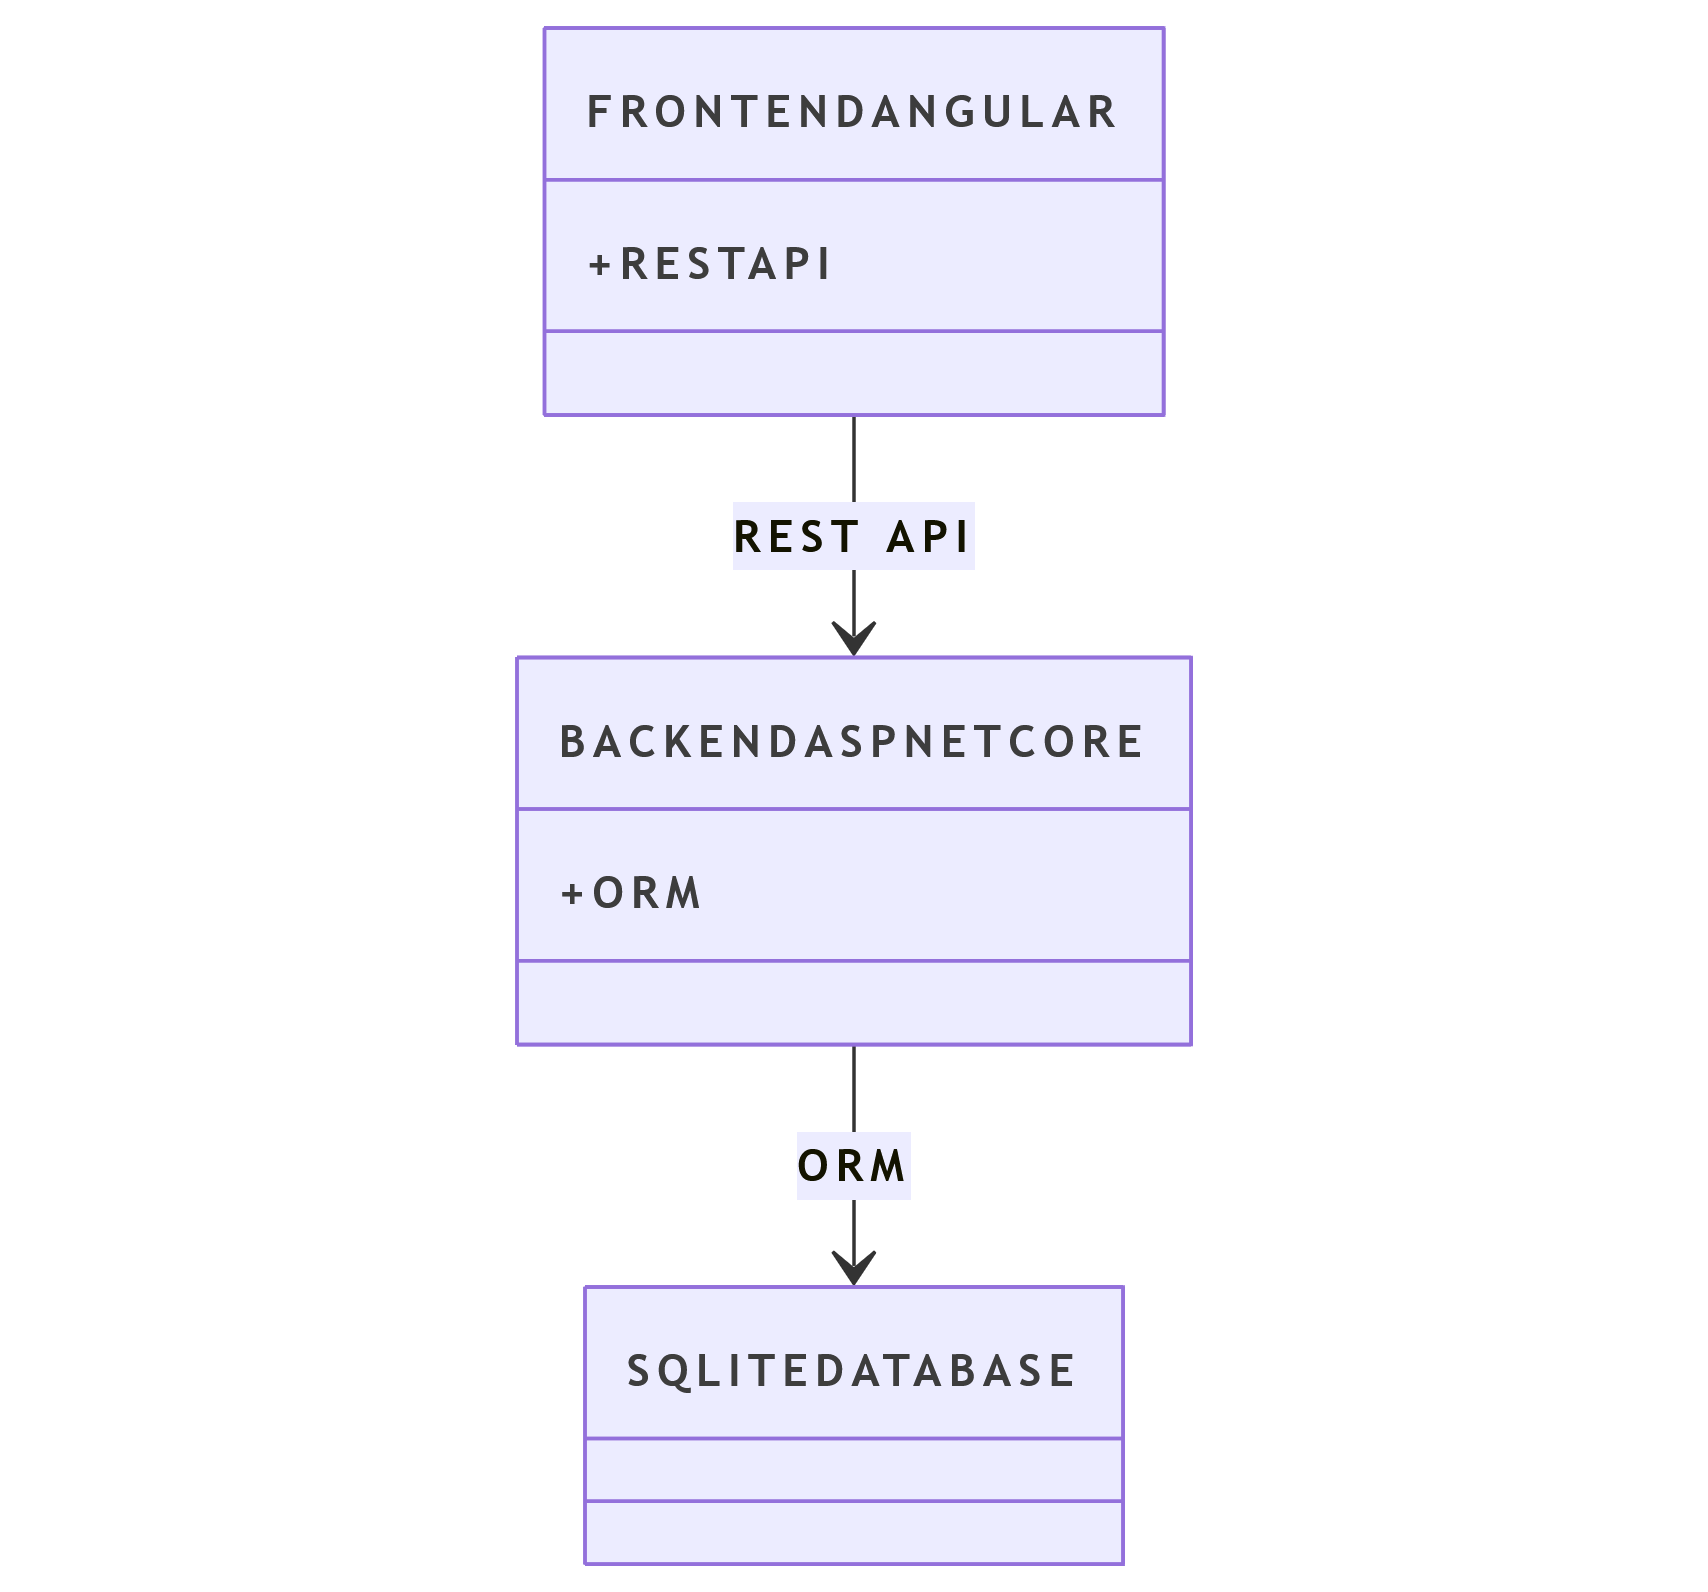
\includegraphics[width=0.8\textwidth]{/chapter3/diagramSystem.png}
	\caption{Uproszczony diagram architektury systemu}
	\label{fig:diagramSystem}
\end{figure}

\begin{figure}[!htb]
	\centering
	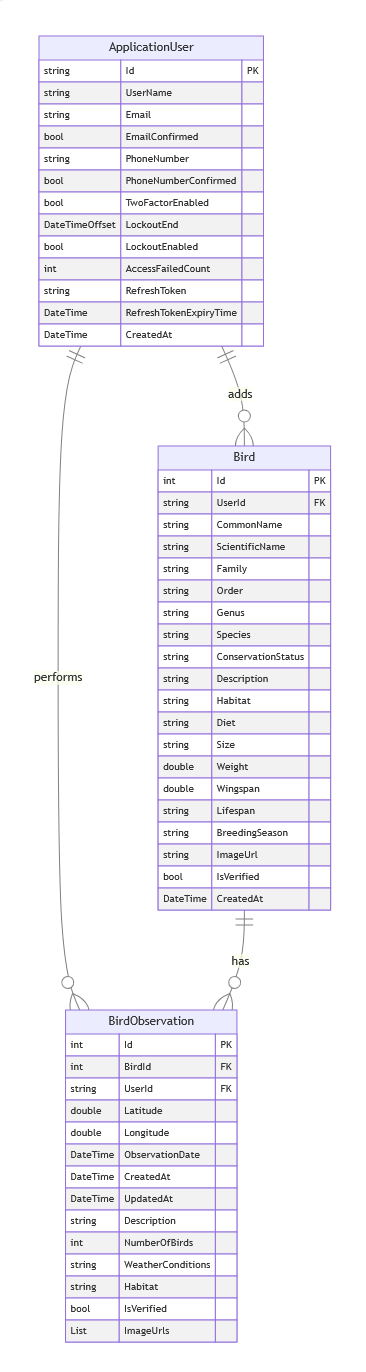
\includegraphics[width=0.4\textwidth]{/chapter3/diagramBazydanych.png}
	\caption{Diagram relacyjny bazy danych}
	\label{fig:diagramBazyDanych}
\end{figure}

% \section{Projekt interfejsu użytkownika}
% \index{Projekt interfejsu użytkownika}

\section{Projekt API}
\index{Projekt API}
API systemu zostało zaprojektowane zgodnie z zasadami REST i składa się z 5 głównych kontrolerów obsługujących różne aspekty funkcjonalności systemu.

\subsection{AuthController}
\begin{itemize}
	\item \texttt{POST /api/auth/login} - logowanie użytkownika
	\item \texttt{POST /api/auth/register} - rejestracja nowego użytkownika
	\item \texttt{POSt /api/auth/refresh-token} - odświeżanie tokenu JWT
	\item \texttt{POST /api/auth/logout} - wylogowanie użytkownika
\end{itemize}

\subsection{BirdsController}
\begin{itemize}
	\item \texttt{GET /api/birds} - pobieranie zweryfikowanych ptaków z paginacją
	\item \texttt{GET /api/birds/all} - pobieranie wszystkich ptaków
	\item \texttt{GET /api/birds/unverified} - pobieranie niezweryfikowanych ptaków
	\item \texttt{GET /api/birds/\{id\}} - pobieranie szczegółów ptaka
	\item \texttt{POST /api/birds} - dodawanie nowego ptaka
	\item \texttt{PUT /api/birds/\{id\}} - aktualizacja danych ptaka
	\item \texttt{DELETE /api/birds/\{id\}} - usuwanie ptaka
	\item \texttt{POST /api/birds/\{id\}/verify} - weryfikacja ptaka
	\item \texttt{GET /api/birds/search} - wyszukiwanie ptaków po nazwie
\end{itemize}

\subsection{BirdObservationsController}
\begin{itemize}
	\item \texttt{GET /api/birdobservations} - pobieranie wszystkich obserwacji z paginacją
	\item \texttt{GET /api/birdobservations/user} - pobieranie obserwacji użytkownika
	\item \texttt{GET /api/birdobservations/\{id\}} - pobieranie szczegółów obserwacji
	\item \texttt{POST /api/birdobservations/} - dodawanie nowej obserwacji
	\item \texttt{PUT /api/birdobservations/\{id\}} - aktualizacja obserwacji
	\item \texttt{DELETE /api/birdobservations/\{id\}} - usuwanie obserwacji
	\item \texttt{POST /api/birdobservations/\{id\}/verify} - weryfikacja obserwacji
	\item \texttt{DELETE /api/birdobservations/\{id\}/images} - usuwanie zdjęć z obserwacji
	\item \texttt{GET /api/birdsobservations/weeks} - pobieranie obserwacji w podziale na tygodnie
\end{itemize}

\subsection{UserManagementController}
\begin{itemize}
	\item \texttt{GET /api/usermanagement} - pobieranie listy użytkowników
	\item \texttt{GET /api/usermanagement/\{id\}} - pobieranie szczegółów użytkownika
	\item \texttt{DELETE /api/usermanagement/\{id\}} - usuwanie użytkownika 
\end{itemize}

\subsection{UserSettingsController}
\begin{itemize}
	\item \texttt{GET /api/usersettings} - pobieranie ustawień użytkownika
	\item \texttt{PUT /api/usersettings} - aktualizacja ustawień użytkownika
\end{itemize}